\documentclass{beamer}
\usepackage[utf8]{inputenc}
\usepackage[english]{babel}
\usepackage[T1]{fontenc}
\usepackage{slide_helper}
\usepackage[inline]{asymptote}
\usepackage{asy_helper}
\usepackage{colortbl}
\usepackage{pgfplots}
\pgfplotsset{compat=1.5} 
\usepgfplotslibrary{statistics}

\begin{asydef}
guide normal_dist(real mu, real sigma, real xmin, real xmax)
{
	real nd_func(real x) { return 1/sqrt(2*pi*sigma*sigma)*exp((-1*(x-mu)*(x-mu))/(2*sigma*sigma)); }
	return graph(nd_func, xmin, xmax);
}

void shade_below(real mu, real sigma, real b, real xmin, real xmax, pen p=orange)
{
	real nd_func(real x) { return 1/sqrt(2*pi*sigma*sigma)*exp((-1*(x-mu)*(x-mu))/(2*sigma*sigma)); }
		
	guide g = graph(nd_func, xmin, b);
	
	filldraw(g -- (b,0) -- cycle, p, black);
	
	draw((xmin,0)--(b,0));
}

void shade_between(real mu, real sigma, real a, real b, pen p=orange)
{
	real nd_func(real x) { return 1/sqrt(2*pi*sigma*sigma)*exp((-1*(x-mu)*(x-mu))/(2*sigma*sigma)); }
		
	guide g = graph(nd_func, a, b);
	
	filldraw((a,0) -- g -- (b,0) -- cycle, p, black);
}

void multiple_nd_curves_example(real std_dev)
{
	size(300, 190, IgnoreAspect);
    
    draw(normal_dist(0, std_dev, -6,6));
    shade_between(0,std_dev,-std_dev,std_dev);
    draw((0,0)--(0,0.45));
    
    label("$\sigma="+format("%#.2f", std_dev)+"$", (-4.2,0.45), Fill(paleyellow));
    
    xaxis(Bottom(), RightTicks(new real[] {-6,-4,-2,0,2,4,6}));
    yaxis(Left(), LeftTicks(size=nan),ymin = 0, ymax = 0.5);
}
\end{asydef}

\newcommand{\prob}[1]{P\left(#1\right)}
\newcommand{\condprob}[2]{\prob{#1~\middle|~#2}}
\newcommand{\comb}[2]{_{#1}C_{#2}}

\title[MATH 1030 - Module 10 - Normal Distribution]{Normal Distribution}

\begin{document}
\begin{frame}
\titlepage
\end{frame}

\begin{frame}
\begin{example}
Consider making popcorn. You put some oil and corn kernels in a pan and start heating.

\vspace{2mm}
For the first few minutes nothing happens, then a few kernels start to pop. A little while later more and more start to pop. This goes one for a minute or so, and the popping gradually tappers off.

\vspace{2mm}
Most of the popping happens in that brief, noisy moment. This demonstrates a typical pattern that is part of many phenomena.
\end{example}
\end{frame}

\begin{frame}[fragile]
\begin{definition}
A \textbf{normal distribution} is a perfectly symmetric, mound-shaped distribution. It is also referred to as a \textbf{normal curve} or a \textbf{bell curve}.
\begin{center}
\begin{asy}
size(320);

shade_below(0, 0.3, 0, -1.5, 1.5);
draw(normal_dist(0, 0.3, -1.5, 1.5));
draw((0,0)--(0,1.45));

xaxis();
//yaxis();

label(minipage("Mean Median Mode", 30),(.8,1.1));
draw((.8,1.25){up}..{left}(0.01,1.4),Arrow);

label("Lower 50\%", (-0.3,0.15));
label("Upper 50\%", (0.3,0.15));

draw((-1,-0.1)--(1,-0.1), Arrows);
label("Curves continues forever in both directions", (0, -0.2));

label(minipage("Curve never touches the $x$-axis", 45), (-1.2,0.15));
\end{asy}
\end{center}
\end{definition}
\end{frame}

\begin{frame}[fragile]
\begin{note}
It is common to use the notation:
\begin{itemize}
\item $\mu = \text{mean}$
\item $\sigma = \text{standard deviation}$
\end{itemize}
\end{note}\pause

\begin{definition}
When $\mu=0$ and $\sigma=1$, the curve is called the \textbf{standard normal distribution}.
\begin{center}
\begin{asy}
size(300, 100, IgnoreAspect);

draw((1,0)--(1,0.5), red);
draw((-1,0)--(-1,0.5), red);

draw(normal_dist(0, 1, -4, 4));
draw((0,0)--(0,0.5));

xaxis(Bottom(), RightTicks(NoZero, size=nan));
yaxis(Left(), LeftTicks(size=nan),ymin = 0, ymax = 0.5);

label("$\mu+\sigma$", (1, 0.45), UnFill);
label("$\mu-\sigma$", (-1, 0.45), UnFill);
\end{asy}
\end{center}
\end{definition}
\end{frame}

\begin{frame}[fragile]
\begin{definition}
The \textbf{empirical rule}, or \textbf{68-95-99.7 rule}, states approximately how much of the area is contained when stepping one, two, or three standard deviations from the mean.
\begin{overprint}
\onslide<1>
One standard deviation from the mean.
\begin{center}
\begin{asy}
size(300, 170, IgnoreAspect);

shade_between(0,1,-1,1);
draw(normal_dist(0, 1, -5, 5));
draw((0,0)--(0,0.45));

label("\Large\textbf{68\%}", (0,0.1), white);

xaxis(Bottom(), RightTicks(new real [] {-4,-3,-2,-1,0,1,2,3,4}, size=nan, ticklabel = new string(real x) { if (x == 0) return "$\mu$"; else return "$" + string(x) + "\sigma$";}));
\end{asy}
\end{center}
\onslide<2>
Two standard deviations from the mean.
\begin{center}
\begin{asy}
size(300, 170, IgnoreAspect);

shade_between(0,1,-2,2);
draw(normal_dist(0, 1, -5, 5));
draw((0,0)--(0,0.45));

label("\Large\textbf{95\%}", (0,0.1), white);

xaxis(Bottom(), RightTicks(new real [] {-4,-3,-2,-1,0,1,2,3,4}, size=nan, ticklabel = new string(real x) { if (x == 0) return "$\mu$"; else return "$" + string(x) + "\sigma$";}));
\end{asy}
\end{center}
\onslide<3>
Three standard deviations from the mean.
\begin{center}
\begin{asy}
size(300, 170, IgnoreAspect);

shade_between(0,1,-3,3);
draw(normal_dist(0, 1, -5, 5));
draw((0,0)--(0,0.45));

label("\Large\textbf{99.7\%}", (0,0.1), white);

xaxis(Bottom(), RightTicks(new real [] {-4,-3,-2,-1,0,1,2,3,4}, size=nan, ticklabel = new string(real x) { if (x == 0) return "$\mu$"; else return "$" + string(x) + "\sigma$";}));
\end{asy}
\end{center}
\onslide<4>
For each standard deviation from the mean.
\begin{center}
\begin{asy}
size(300, 170, IgnoreAspect);

shade_between(0, 1,-4, -3, white);
shade_between(0, 1,-3, -2, green);
shade_between(0, 1,-2, -1, royalblue);
shade_between(0, 1,-1,  0, orange);
shade_between(0, 1, 0,  1, fuchsia);
shade_between(0, 1, 1,  2, purple);
shade_between(0, 1, 2,  3, mediumcyan);
shade_between(0, 1, 3,  4, yellow);

draw((0,0)--(0,0.45));

real nd_func(real x, real mu, real sigma) { return 1/sqrt(2*pi*sigma*sigma)*exp((-1*(x-mu)*(x-mu))/(2*sigma*sigma)); }

void sndlabel(string s, pair pt, real offset=0.01)
{
	pair c = (pt.x, nd_func(pt.x, 0, 1) + offset);
	
	draw(pt -- c, EndArrow);
	label(s , pt, UnFill());
}

sndlabel("34\%",   (-0.5, 0.43));
sndlabel("34\%",   ( 0.5, 0.43));
sndlabel("13\%",   (-1.5, 0.25));
sndlabel("13\%",   ( 1.5, 0.25));
sndlabel("2.35\%", (-2.5, 0.15));
sndlabel("2.35\%", ( 2.5, 0.15));
sndlabel("0.1\%",  (-3.5, 0.05));
sndlabel("0.1\%",  ( 3.5, 0.05));

xaxis(Bottom(), RightTicks(new real [] {-4,-3,-2,-1,0,1,2,3,4}, size=nan, ticklabel = new string(real x) { if (x == 0) return "$\mu$"; else return "$" + string(x) + "\sigma$";}));
\end{asy}
\end{center}
\end{overprint}
\end{definition}
\end{frame}

\begin{frame}
\begin{definition}
A \textbf{z-score} is a measure of the number of standard deviations a particular data point is away from the mean. It is calculated with:
\begin{equation*}
z=\dfrac{\left(\text{data point}\right)-\left(\text{mean}\right)}{\text{standard deviation}}=\dfrac{x-\mu}{\sigma}
\end{equation*}
\end{definition}\pause

\begin{example}
On a college entrance exam, the mean was 70, and the standard deviation was 8. Rose scored a 85, what is her $z$-score?\pause

\begin{equation*}
z=\dfrac{x-\mu}{\sigma}\pause=\dfrac{85-70}{8}\pause\approx 1.875
\end{equation*}

\vspace{-4.3mm}
\end{example}\pause

\begin{example}
On the same exam, George has a $z$-score of $-1.3$. What was his score?\pause
\begin{equation*}
z=\dfrac{x-\mu}{\sigma}\pause
\quad\Rightarrow\quad
z\sigma=x-\mu\pause
\quad\Rightarrow\quad
x=z\sigma+\mu\pause = \left(-1.3\right)\left(8\right)+70=59.6
\end{equation*}

\vspace{-4.5mm}
\end{example}
\end{frame}

\begin{frame}
\begin{example}
The mean on a exam was 82, with a standard deviation of 7 points. An \textquote{A} on the exam is a 93, what is the $z$-score?\pause
\begin{equation*}
z=\dfrac{x-\mu}{\sigma}=\dfrac{93-82}{7}\approx 1.57
\end{equation*}
\end{example}\pause

\begin{note}
We know from the empirical rule that roughly 68\% of the scores fall within one standard deviation of the mean. This means that 68\% of the students scored between 75 and 89.\pause

\vspace{2mm}
Moreover, we know that roughly 95\% of the scores fall within two standard deviations of the mean. Which means that $95\%-68\%=32\%$ of the scores are more than one standard deviation from the mean, but less than two. \pause

\vspace{2mm}
Since the curve is symmetric, we know that 16\% of the students scored between 89 and 96, as well as 16\% between 68 and 75
\end{note}
\end{frame}

\begin{frame}
\begin{note}
Visual representations of data, such as histograms can tell you if data is roughly normal or not.
\end{note}\pause

\begin{example}
This data is not a normal distribution.

\begin{center}
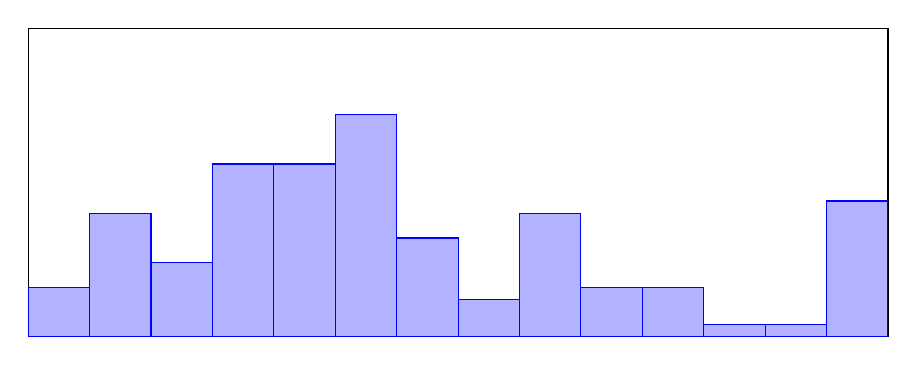
\begin{tikzpicture}
\begin{axis}[
small,
height=5.5cm,
width=12.5cm,
enlarge x limits=false,
enlarge y limits=false,
ybar interval,
%ymajorgrids=true,
%ylabel={Frequency},
%xlabel={Weights (pounds)},
%x tick label style={rotate=40,anchor=east},
%xtick={120,140,...,1000},
%ytick={0,5,...,1000},
xtick=\empty,
ytick=\empty,
ymin=0,
ymax=25,
%xmin=120,
%xmax=280,
%xticklabel style={/pgf/number format/.cd,fixed,precision=0},
%xticklabel=
%\pgfmathprintnumber\tick--\pgfmathprintnumber\nexttick
]
\addplot+ [hist={bins=14}]
table [row sep=\\,y index=0] {
data\\
121\\ 131\\ 131\\ 130\\ 138\\ 144\\ 147\\ 142\\ 136\\ 141\\ 141\\ 140\\ 138\\ 138\\ 136\\ 140\\ 148\\ 145\\ 153\\ 157\\ 161\\ 155\\ 160\\ 156\\ 157\\ 155\\ 156\\ 161\\ 150\\ 156\\ 160\\ 157\\ 151\\ 155\\ 174\\ 175\\ 171\\ 168\\ 176\\ 168\\ 174\\ 176\\ 176\\ 172\\ 175\\ 172\\ 176\\ 166\\ 175\\ 176\\ 168\\ 175\\ 168\\ 178\\ 178\\ 169\\ 169\\ 170\\ 172\\ 178\\ 171\\ 173\\ 181\\ 183\\ 186\\ 189\\ 188\\ 180\\ 187\\ 192\\ 185\\ 188\\ 188\\ 182\\ 207\\ 203\\ 207\\ 207\\ 205\\ 208\\ 208\\ 204\\ 216\\ 214\\ 216\\ 221\\ 211\\ 212\\ 223\\ 236\\ 230\\ 226\\ 232\\ 225\\ 230\\ 248\\ 245\\ 265\\ 267\\ 269\\ 269\\ 269\\ 269\\ 269\\ 269\\ 269\\ 269\\ 269\\
};
\end{axis}
\end{tikzpicture}
\end{center}
\end{example}
\end{frame}

\begin{frame}
\begin{definition}
A \textbf{density curve} is an idealized representation of a distribution in which the area under the curve is defined to be one.
\end{definition}\pause

\begin{note}
A density curve does not need to be normal, but the normal density curve will be of the most use.
\end{note}\pause

\begin{note}
We know from the Empirical rule that roughly two-thirds of the data in a normal distribution falls within one standard deviation of the mean.

\vspace{2mm}
With a normal density curve, this means that about 68\% of the total area under the curve is within $z$-scores of $\pm1$.
\end{note}
\end{frame}

\begin{frame}[fragile]
\begin{example}
Notice that as the standard deviation increases, the curve gets flatter. This is because 68\% of the area always falls within a single standard deviation of the mean.
\begin{overprint}
\onslide<+>
\begin{center}
\begin{asy}
multiple_nd_curves_example(1.0);
\end{asy}
\end{center}
\onslide<+>
\begin{center}
\begin{asy}
multiple_nd_curves_example(1.25);
\end{asy}
\end{center}
\onslide<+>
\begin{center}
\begin{asy}
multiple_nd_curves_example(1.5);
\end{asy}
\end{center}
\onslide<+>
\begin{center}
\begin{asy}
multiple_nd_curves_example(1.75);
\end{asy}
\end{center}
\onslide<+>
\begin{center}
\begin{asy}
multiple_nd_curves_example(2.0);
\end{asy}
\end{center}
\onslide<+>
\begin{center}
\begin{asy}
multiple_nd_curves_example(2.25);
\end{asy}
\end{center}
\onslide<+>
\begin{center}
\begin{asy}
multiple_nd_curves_example(2.5);
\end{asy}
\end{center}
\onslide<+>
\begin{center}
\begin{asy}
multiple_nd_curves_example(2.75);
\end{asy}
\end{center}
\onslide<+>
\begin{center}
\begin{asy}
multiple_nd_curves_example(3.0);
\end{asy}
\end{center}
\end{overprint}
\end{example}
\end{frame}

\begin{frame}[fragile]
\begin{definition}
An \textbf{inflection point} is where a curve changes from being concave up to concave down, or vice versa
\end{definition}\pause

\begin{note}
A normal density curve always has two inflection points, each one standard deviation from the mean.
\begin{center}
\begin{asy}
size(300, 140, IgnoreAspect);

real nd_func(real x, real mu, real sigma) { return 1/sqrt(2*pi*sigma*sigma)*exp((-1*(x-mu)*(x-mu))/(2*sigma*sigma)); }

draw(normal_dist(0, 1, -5, 5));
draw((0,0)--(0,nd_func(0,0,1)));

draw((1,0) -- (1,0.45), red);
draw((0,nd_func(1,0,1)) -- (1,nd_func(1,0,1)), red);
dot((1,nd_func(1,0,1)), red);

label("Inflection point", (1,nd_func(1,0,1)), E);

draw((-1,0) -- (-1,0.45), red);
draw((0,nd_func(-1,0,1)) -- (-1,nd_func(-1,0,1)), red);
dot((-1,nd_func(-1,0,1)), red);

label("Inflection point", (-1,nd_func(-1,0,1)), W);

label("Concave up", (2,nd_func(2,0,1)), E);
label("Concave up", (-2,nd_func(-2,0,1)), W);

label("Concave down", (0,nd_func(0,0,1)), N);

xaxis(Bottom(), RightTicks(new real [] {-4,-3,-2,-1,0,1,2,3,4}, size=nan, ticklabel = new string(real x) { if (x == 0) return "$\mu$"; else return "$" + string(x) + "\sigma$";}));
\end{asy}
\end{center}
\end{note}
\end{frame}

\begin{frame}[fragile]
\begin{example}
Estimate the standard deviation of the distribution represented by the histogram.
\begin{overprint}
\onslide<+>
\begin{center}
\begin{asy}
size(300, 135, IgnoreAspect);

real[] freq = {0, 0.8, 1.4, 2.7, 5.2, 8, 12, 15, 16, 15.7, 10, 7.8, 3.9, 1.4, 0.8, 0.4, 0.1};

// draw histogram
path rect(pair a, pair b)
{
	return a -- (a.x, b.y) -- b -- (b.x, a.y) -- cycle;
}
real start = 0.34;
real end = 0.68;
real width = abs(end-start)/freq.length;
for(int i = 0; i < freq.length; ++i)
{
	pen p = mediumgray;
	filldraw(rect(start + (i*width,0), (start + (i+1)*width, abs(freq[i]))), p, black);
}

xaxis(Bottom(), RightTicks(new real[] {0.35, 0.40, 0.45, 0.50, 0.55, 0.60, 0.65}, size=nan));
yaxis(Left(), LeftTicks(new real[] {2, 4, 6, 8, 10, 12, 14, 16, 18, 20}, size=nan, ticklabel = new string(real x) { return "$" + string(x) + "\%$";}), ymax=18);
\end{asy}
\end{center}
\onslide<+>
\begin{center}
\begin{asy}
size(300, 135, IgnoreAspect);

// negative numbers mean color the bars
real[] freq = {0, 0.8, 1.4, 2.7, 5.2, 8, 12, 15, 16, 15.7, 10, 7.8, 3.9, 1.4, 0.8, 0.4, 0.1};

// draw histogram
path rect(pair a, pair b)
{
	return a -- (a.x, b.y) -- b -- (b.x, a.y) -- cycle;
}
real start = 0.34;
real end = 0.68;
real width = abs(end-start)/freq.length;
for(int i = 0; i < freq.length; ++i)
{
	pen p = mediumgray;
		
	filldraw(rect(start + (i*width,0), (start + (i+1)*width, abs(freq[i]))), p, black);
}

// draw density curve
real mu = 0.5;
real sigma = 0.05;
real h = 16;
real density(real x)
{
	real scale = h/(1/sqrt(2*pi*sigma*sigma));
	return scale * 1/sqrt(2*pi*sigma*sigma)*exp((-1*(x-mu)*(x-mu))/(2*sigma*sigma));
}
draw(graph(density, start, end), red+1bp);

xaxis(Bottom(), RightTicks(new real[] {0.35, 0.40, 0.45, 0.50, 0.55, 0.60, 0.65}, size=nan));
yaxis(Left(), LeftTicks(new real[] {2, 4, 6, 8, 10, 12, 14, 16, 18, 20}, size=nan, ticklabel = new string(real x) { return "$" + string(x) + "\%$";}), ymax=18);
\end{asy}
\end{center}
First, draw a density curve that fits the histogram fairly well.
\onslide<+>
\begin{center}
\begin{asy}
size(300, 135, IgnoreAspect);

// negative numbers mean color the bars
real[] freq = {0, 0.8, 1.4, 2.7, 5.2, 8, 12, 15, 16, 15.7, 10, 7.8, 3.9, 1.4, 0.8, 0.4, 0.1};

// draw histogram
path rect(pair a, pair b)
{
	return a -- (a.x, b.y) -- b -- (b.x, a.y) -- cycle;
}
real start = 0.34;
real end = 0.68;
real width = abs(end-start)/freq.length;
for(int i = 0; i < freq.length; ++i)
{
	pen p = mediumgray;
		
	filldraw(rect(start + (i*width,0), (start + (i+1)*width, abs(freq[i]))), p, black);
}

// draw density curve
real mu = 0.5;
real sigma = 0.05;
real h = 16;
real density(real x)
{
	real scale = h/(1/sqrt(2*pi*sigma*sigma));
	return scale * 1/sqrt(2*pi*sigma*sigma)*exp((-1*(x-mu)*(x-mu))/(2*sigma*sigma));
}
draw(graph(density, start, end), red+1bp);

// draw inflection points
dot((mu+sigma, density(mu+sigma)), black);
dot((mu-sigma, density(mu-sigma)), black);

xaxis(Bottom(), RightTicks(new real[] {0.35, 0.40, 0.45, 0.50, 0.55, 0.60, 0.65}, size=nan));
yaxis(Left(), LeftTicks(new real[] {2, 4, 6, 8, 10, 12, 14, 16, 18, 20}, size=nan, ticklabel = new string(real x) { return "$" + string(x) + "\%$";}), ymax=18);
\end{asy}
\end{center}
Next, estimate the inflections points, as well as the mean.

\vspace{2mm}
In this case, we have $\mu\approx 0.5$ and $\sigma\approx0.05$.

\vspace{2mm}
(The actual statistics are:  $\text{mean = 0.04988}$ and $\text{std.\ dev.} = 0.4997$.)
\onslide<+>
\begin{center}
\begin{asy}
size(300, 135, IgnoreAspect);

// negative numbers mean color the bars
real[] freq = {0, 0.8, 1.4, 2.7, 5.2, -8, -12, -15, -16, -15.7, -10, 7.8, 3.9, 1.4, 0.8, 0.4, 0.1};

// draw histogram
path rect(pair a, pair b)
{
	return a -- (a.x, b.y) -- b -- (b.x, a.y) -- cycle;
}
real start = 0.34;
real end = 0.68;
real width = abs(end-start)/freq.length;
for(int i = 0; i < freq.length; ++i)
{
	pen p = mediumgray;
	if (freq[i] < 0)
	{
		p = royalblue;
		
		// also label colored bars
		if (abs(freq[i-1]) > abs(freq[i]))
			label("$" + string(abs(freq[i])) + "\%$", (start + (i+1)*width, abs(freq[i])), E, p);
		else
			if (abs(freq[i+1]) < abs(freq[i]))
				label("$" + string(abs(freq[i])) + "\%$", (start + (i)*width + width/2, abs(freq[i])), N, p);
			else
				label("$" + string(abs(freq[i])) + "\%$", (start + (i)*width, abs(freq[i])), W, p);
	}
	
	filldraw(rect(start + (i*width,0), (start + (i+1)*width, abs(freq[i]))), p, black);
}

// draw density curve
real mu = 0.5;
real sigma = 0.05;
real h = 16;
real density(real x)
{
	real scale = h/(1/sqrt(2*pi*sigma*sigma));
	return scale * 1/sqrt(2*pi*sigma*sigma)*exp((-1*(x-mu)*(x-mu))/(2*sigma*sigma));
}
draw(graph(density, start, end), red+1bp);

// draw inflection points
dot((mu+sigma, density(mu+sigma)), black);
dot((mu-sigma, density(mu-sigma)), black);

xaxis(Bottom(), RightTicks(new real[] {0.35, 0.40, 0.45, 0.50, 0.55, 0.60, 0.65}, size=nan));
yaxis(Left(), LeftTicks(new real[] {2, 4, 6, 8, 10, 12, 14, 16, 18, 20}, size=nan, ticklabel = new string(real x) { return "$" + string(x) + "\%$";}), ymax=18);
\end{asy}
\end{center}
We can estimate how much of the graph is within one standard deviation by estimating the heights of the colored bins.

\vspace{-4mm}
\begin{equation*}
\tfrac{8}{2}+12+15+16+15.75+\tfrac{10}{2}=67.7
\end{equation*}

\vspace{-2mm}
This is remarkably close to the 68\% the Empirical rule gives.
\end{overprint}
\end{example}
\end{frame}

\begin{frame}[fragile]
\begin{example}\label{ex:coin flips}
Suppose you flip 8 coins and record the results. The histogram shows the results of performing this experiment 256 times.
\begin{overprint}
\onslide<+>
\begin{center}
\begin{asy}
size(300, 100, IgnoreAspect);

// negative numbers mean color the bars
real[] freq = {1, 8, 28, 56, 70, 56, 28, 8, 1};

// draw histogram
path rect(pair a, pair b)
{
	return a -- (a.x, b.y) -- b -- (b.x, a.y) -- cycle;
}
real start = -0.5;
real end = 8.5;
real width = abs(end-start)/freq.length;
for(int i = 0; i < freq.length; ++i)
{
	pen p = mediumgray;
	if (freq[i] < 0)
	{
		p = royalblue;
	}
	
	filldraw(rect(start + (i*width,0), (start + (i+1)*width, abs(freq[i]))), p, black);
}

xaxis("Number of tails", Bottom(), RightTicks(new real[] {0, 1, 2, 3, 4, 5, 6, 7, 8}, new real[] {0.5, 1.5, 2.5, 3.5, 4.5, 5.5, 6.5, 7.5, 8.5}), xmin=-0.5, xmax=9);
yaxis("Frequency", Left(), LeftTicks(new real[] {10, 20, 30, 40, 50, 60, 70}, new real[] {5, 15, 25, 35, 45, 55, 65, 75}), ymax=75);
\end{asy}
\end{center}
\onslide<+>
\begin{center}
\begin{asy}
size(300, 100, IgnoreAspect);

// negative numbers mean color the bars
real[] freq = {1, 8, 28, 56, 70, 56, 28, 8, 1};

// draw histogram
path rect(pair a, pair b)
{
	return a -- (a.x, b.y) -- b -- (b.x, a.y) -- cycle;
}
real start = -0.5;
real end = 8.5;
real width = abs(end-start)/freq.length;
for(int i = 0; i < freq.length; ++i)
{
	pen p = mediumgray;
	if (freq[i] < 0)
	{
		p = royalblue;
	}
	
	filldraw(rect(start + (i*width,0), (start + (i+1)*width, abs(freq[i]))), p, black);
}

xaxis("Number of tails", Bottom(), RightTicks(new real[] {0, 1, 2, 3, 4, 5, 6, 7, 8}, new real[] {0.5, 1.5, 2.5, 3.5, 4.5, 5.5, 6.5, 7.5, 8.5}), xmin=-0.5, xmax=9);
yaxis("Frequency", Left(), LeftTicks(new real[] {10, 20, 30, 40, 50, 60, 70}, new real[] {5, 15, 25, 35, 45, 55, 65, 75}), ymax=75);
\end{asy}
\end{center}
One way to calculate the probability that exactly three tails are flipped is:
\begin{equation*}
\prob{\text{3 tails}} = \dfrac{\comb{8}{3}}{2^8} = \dfrac{56}{256} \approx 0.2188
\end{equation*}
\onslide<+>
\begin{center}
\begin{asy}
size(300, 100, IgnoreAspect);

// negative numbers mean color the bars
real[] freq = {1, 8, 28, -56, 70, 56, 28, 8, 1};

// draw histogram
path rect(pair a, pair b)
{
	return a -- (a.x, b.y) -- b -- (b.x, a.y) -- cycle;
}
real start = -0.5;
real end = 8.5;
real width = abs(end-start)/freq.length;
for(int i = 0; i < freq.length; ++i)
{
	pen p = mediumgray;
	if (freq[i] < 0)
	{
		p = royalblue;
	}
	
	filldraw(rect(start + (i*width,0), (start + (i+1)*width, abs(freq[i]))), p, black);
	
	//if (i > 0)
	//draw((start+(i-1)*width+width/2, abs(freq[i-1]))--(start+(i)*width+width/2,abs(freq[i])),red+1bp);
}

xaxis("Number of tails", Bottom(), RightTicks(new real[] {0, 1, 2, 3, 4, 5, 6, 7, 8}, new real[] {0.5, 1.5, 2.5, 3.5, 4.5, 5.5, 6.5, 7.5, 8.5}), xmin=-0.5, xmax=9);
yaxis("Frequency", Left(), LeftTicks(new real[] {10, 20, 30, 40, 50, 60, 70}, new real[] {5, 15, 25, 35, 45, 55, 65, 75}), ymax=75);
\end{asy}
\end{center}
A second way is to approximate the heights of each box and divide the area of the colored box by the areas of all the boxes:

\vspace{-6mm}
\begin{equation*}
\prob{\text{3 tails}} = \dfrac{55}{1+8+28+55+70+55+28+8+1} = \dfrac{55}{254} \approx 0.2165
\end{equation*}
\onslide<+>
\begin{center}
\begin{asy}
size(300, 100, IgnoreAspect);

// negative numbers mean color the bars
real[] freq = {1, 8, 28, -56, 70, 56, 28, 8, 1};

// draw histogram
path rect(pair a, pair b)
{
	return a -- (a.x, b.y) -- b -- (b.x, a.y) -- cycle;
}
real start = -0.5;
real end = 8.5;
real width = abs(end-start)/freq.length;
for(int i = 0; i < freq.length; ++i)
{
	pen p = mediumgray;
	//if (freq[i] < 0)
	//{
	//	p = royalblue;
	//}
	
	filldraw(rect(start + (i*width,0), (start + (i+1)*width, abs(freq[i]))), p, black);
	
	if (i > 0)
	draw((start+(i-1)*width+width/2, abs(freq[i-1]))--(start+(i)*width+width/2,abs(freq[i])),red+1bp);
}

pair mid(int i) { return (i+0.5, abs(freq[i]) + (abs(freq[i+1])-abs(freq[i]))/2); }

path p = (2.5,0) -- mid(2) -- (3, abs(freq[3])) -- mid(3) -- (3.5,0) -- cycle;
filldraw(p, royalblue, black);

for(int i = 0; i < freq.length; ++i)
{
	if (i > 0)
	draw((start+(i-1)*width+width/2, abs(freq[i-1]))--(start+(i)*width+width/2,abs(freq[i])),red+1bp);
}

real area = 0;
for(int i = 0; i < freq.length - 1; ++i)
{
	real cur = abs(freq[i]);
	real nxt = abs(freq[i+1]);
	
	real ths = cur + 0.5 * abs(nxt-cur);
	area = area + ths;
}

//write("Area under entire curve = " + string(area));

real left = mid(2).y;
real mid = abs(freq[3]);
real right = mid(3).y;

area = left + 0.5*0.5*(mid-left) + (mid-left) + 0.5*0.5*(right-mid);
//write("Colored area = " + string(area));

xaxis("Number of tails", Bottom(), RightTicks(new real[] {0, 1, 2, 3, 4, 5, 6, 7, 8}, new real[] {0.5, 1.5, 2.5, 3.5, 4.5, 5.5, 6.5, 7.5, 8.5}), xmin=-0.5, xmax=9);
yaxis("Frequency", Left(), LeftTicks(new real[] {10, 20, 30, 40, 50, 60, 70}, new real[] {5, 15, 25, 35, 45, 55, 65, 75}), ymax=75);
\end{asy}
\end{center}
A third way is to draw an approximate normal curve. Then, the area from 2.5 to 3.5 relates to the probability of the event.
\begin{equation*}
\prob{\text{3 tails}} = \dfrac{\text{Area from 2.5 to 3.5}}{\text{Total area under curve}} = \dfrac{61.25}{324} \approx 0.1890
\end{equation*}
\onslide<+>
\begin{center}
\begin{asy}
size(300, 100, IgnoreAspect);

// negative numbers mean color the bars
real[] freq = {1, 8, 28, -56, 70, 56, 28, 8, 1};

// draw histogram
path rect(pair a, pair b)
{
	return a -- (a.x, b.y) -- b -- (b.x, a.y) -- cycle;
}
real start = -0.5;
real end = 8.5;
real width = abs(end-start)/freq.length;
for(int i = 0; i < freq.length; ++i)
{
	pen p = mediumgray;
	//if (freq[i] < 0)
	//{
	//	p = royalblue;
	//}
	
	filldraw(rect(start + (i*width,0), (start + (i+1)*width, abs(freq[i]))), p, black);
}

// draw density curve
real mu = 4;
real sigma = 1.5;
real h = 70;
real density(real x)
{
	real scale = h/(1/sqrt(2*pi*sigma*sigma));
	return scale * 1/sqrt(2*pi*sigma*sigma)*exp((-1*(x-mu)*(x-mu))/(2*sigma*sigma));
}

fill((2.5,0) -- graph(density, 2.5, 3.5) -- (3.5,0) -- cycle, royalblue);
draw(graph(density, start, end), red+1bp);

dot((2.5, density(2.5)));
dot((5.5, density(5.5)));

xaxis("Number of tails", Bottom(), RightTicks(new real[] {0, 1, 2, 3, 4, 5, 6, 7, 8}, new real[] {0.5, 1.5, 2.5, 3.5, 4.5, 5.5, 6.5, 7.5, 8.5}), xmin=-0.5, xmax=9);
yaxis("Frequency", Left(), LeftTicks(new real[] {10, 20, 30, 40, 50, 60, 70}, new real[] {5, 15, 25, 35, 45, 55, 65, 75}), ymax=75);
\end{asy}
\end{center}
The better we draw the density curve, the better our approximation.

\begin{equation*}
\prob{\text{3 tails}} = \dfrac{\text{Area from 2.5 to 3.5}}{\text{Total area under curve}} = \dfrac{55.478}{262.075} \approx 0.2117
\end{equation*}
\end{overprint}
\end{example}
\end{frame}

\begin{frame}[fragile]
\begin{definition}
The area of a region under the standard normal density curve is the probability of a data point falling in that region.
\end{definition}\pause

\begin{note}
To actually calculate the area of density curve is not easy, this is why either a table or a computer is usually used.
\end{note}\pause

\begin{example}
Here is a section of a Standard Normal Probability table.

\vspace{-3mm}
\begin{center}
\definecolor{amethyst}{rgb}{0.6, 0.4, 0.8}
\definecolor{peridot}{rgb}{0.9, 0.89, 0.0}
\definecolor{periwinkle}{rgb}{0.8, 0.8, 1.0}
\begin{tabular}{r|rrrrrrrrrr}
$z$&0.00&0.01&0.02&0.03&0.04&0.05\\\hline
1.4&0.9192&0.9207&0.9222&0.9236&0.9251&0.9265\\
1.5&0.9332&0.9345&0.9357&0.9370&0.9382&0.9394\\
1.6&0.9452&0.9463&0.9474&\only<4->{\cellcolor{periwinkle}}0.9484&0.9495&0.9505\\
1.7&0.9554&0.9564&0.9573&0.9582&0.9591&0.9599\\
1.8&0.9641&0.9649&0.9656&0.9664&0.9671&0.9678\\
\end{tabular}
\end{center}
What is the probability that $z\leq 1.63$? \visible<4->{$\prob{z\leq 1.63} = 0.9484$}
\end{example}
\end{frame}

\begin{frame}[fragile]
\begin{example}
\begin{center}
\begin{asy}
size(300, 50, IgnoreAspect);

draw(normal_dist(0, 1, -4, 4));
shade_between(0,1,-4,0.8);
//draw((0,0)--(0,0.5));

xaxis(Bottom(), RightTicks(new real[] {0,0.8}, ticklabel=new string(real x) { if (x==0) return "0"; else return "$x$";}, size=nan));
//yaxis(Left(), LeftTicks(size=nan),ymin = 0, ymax = 0.5);
\end{asy}
\end{center}
The area of the shaded region is the probability that a $z$ score is less than or equal to $x$, $\prob{z\leq x}$.
\end{example}\pause

\begin{example}
\begin{center}
\begin{asy}
size(300, 50, IgnoreAspect);

draw(normal_dist(0, 1, -4, 4));
shade_between(0,1,-0.8,4);
//draw((0,0)--(0,0.5));

xaxis(Bottom(), RightTicks(new real[] {0,-0.8}, ticklabel=new string(real x) { if (x==0) return "0"; else return "$x$";}, size=nan));
//yaxis(Left(), LeftTicks(size=nan),ymin = 0, ymax = 0.5);
\end{asy}
\end{center}
The area of the shaded region is the probability that a $z$ score is greater than or equal to $x$, $\prob{z\geq x}$. Can also be calculated as $1 - \prob{z\leq x}$.
\end{example}
\end{frame}

\begin{frame}[fragile]
\begin{example}
\begin{center}
\begin{asy}
size(300, 50, IgnoreAspect);

draw(normal_dist(0, 1, -4, 4));
shade_between(0,1,-0.7,1.2);
//draw((0,0)--(0,0.5));

xaxis(Bottom(), RightTicks(new real[] {0,-0.7, 1.2}, ticklabel=new string(real x) { if (x==0) return "0"; else if (x < 0) return "$x_1$"; else return "$x_2$";}, size=nan));
//yaxis(Left(), LeftTicks(size=nan),ymin = 0, ymax = 0.5);
\end{asy}
\end{center}
The area of the shaded region is the probability that a $z$ score lies between $x_1$ and $x_2$, $\prob{x_1\leq z\leq x_2}$. 

\vspace{2mm}
Can also be calculated as $\prob{x\leq x_2} - \prob{z\leq x_1}$.
\end{example}\pause

\begin{note}
It is always a good idea to sketch a picture of the normal density curve you are dealing with, so that you make sure you're finding the proper area.
\end{note}
\end{frame}

\begin{frame}
\begin{note}
Always remember that Standard Normal Probability tables and programs are dealing with the standard normal distribution, that is $\mu=0$ and $\sigma=1$.\pause

\vspace{2mm}
To use such a table on an arbitary density function, you need to \textbf{standardize} the distribution by calculating $z$-scores.\pause

\vspace{2mm}
This works because all normal distribution curves have the same basic shape and the $z$-score gives a relative distance from the mean.
\end{note}\pause

\begin{block}{Recall}
The $z$-score is:
\begin{equation*}
z=\dfrac{x-\mu}{\sigma}
\end{equation*}
\end{block}\pause
\begin{note}
In statistics, the term \textquote{unusual} often refers to an event with probability less than 5\% ($p<0.05$).
\end{note}
\end{frame}

\begin{frame}
\begin{example}
Let us return to example~\ref{ex:coin flips}, where we were looking for the probability that we would get exactly three tails. After fitting an approximate normal curve, we needed the area between 2.5 and 3.5.\pause 

\vspace{2mm}
These values have the $z$-scores:
\begin{equation*}
z_{2.5} = \dfrac{x-\mu}{\sigma} = \dfrac{2.5-4}{1.5} = -1
\quad\text{and}\quad
z_{3.5} = \dfrac{3.5-4}{1.5} = -0.3333
\end{equation*}\pause
So, then
\begin{equation*}
\begin{aligned}
\prob{-1\leq z\leq -0.3333} &= \prob{z\leq -0.3333} - \prob{z\leq -1} \\
&= 0.369441-0.158655 \\
&=0.210786
\end{aligned}
\end{equation*}
\end{example}\pause

\begin{note}
It's not at all unusual to flip eight coins and get three tails.
\end{note}
\end{frame}

\begin{frame}
\begin{example}
A candy company sells small bags of candy. While they attempt to keep the number of pieces in each bag the same, small differences occur because of variation in the packaging process. A quality control expert in the factory determined that the mean number of pieces in each bag is normally distributed, with a mean of 57.3 and a standard deviation of 1.6.

\vspace{2mm}
Let us find the probability that we will purchase a bag with 55 or fewer pieces of candy.\pause

\vspace{2mm}
The $z$-score is
\begin{equation*}
z=\dfrac{x-\mu}{\sigma}=\dfrac{55-57.3}{1.6}=-1.4375
\end{equation*}\pause
Thus,
\begin{equation*}
\prob{z\leq-1.4375} = 0.075288
\end{equation*}
A roughly 8\% chance, it would be rare, but not unusual.
\end{example}
\end{frame}

\begin{frame}
\begin{example}
Suppose that a fictional scientist measured the resting body temperature for a large number of people. She found that the mean is $\degrees{98.25}$F and the standard deviation is $\degrees{0.73}$F.

\vspace{2mm}
Johnny \textquote{Hothead} Rico has a resting body temperature of $\degrees{100}$F. Would you consider this unusual?\pause

\vspace{2mm}
Johnny's $z$-score is
\begin{equation*}
z=\dfrac{x-\mu}{\sigma}=\dfrac{100-98.25}{0.73} = 2.3972
\end{equation*}\pause
So, the probability that someone has a resting body temperature $\geq 100$ is
\begin{equation*}
\prob{z\geq 2.3972}=1-\prob{z\leq 2.3972} = 1-0.99174 = 0.00826
\end{equation*}
Johnny is pretty unusual, but don't let him hear you say that.
\end{example}
\end{frame}
\end{document}
